% This is LLNCS.DEM the demonstration file of
% the LaTeX macro package from Springer-Verlag
% for Lecture Notes in Computer Science,
% version 2.3 for LaTeX2e
%
% The infinite quirkiness of TekMaker ....
% ... to get it to fully update, need to hit F1 a few times,
% ... then F11 a few times (for bibliography),
% ... then F1 a bunch more times
% ... .... and then the .pdf catches up to all the edits
% ...	weird that it takes multiple cycles w/ human action ...
% ...
% ...	or maybe this works ..
%...	you can use hotkeys to run pdflatex and bibtex with F6 and F11 on your keyboard
%... 	respectively, so pressing F6 F11 F6 F6 one at a time (and waiting for texmaker to 
% ...	finish each time) you will update everything in your document
% ...
% ... file needed in same directory :
% ...	llncs.cls
% ...	splncs.bst
% ...	pedestrianreferences.bib (bibliography)
%
\documentclass{llncs}
%
% additional packages added to comply wth format recommendations
%
\usepackage{makeidx}  % allows for indexgeneration
\usepackage[strings]{underscore} % allows underscore
\usepackage{float} % position tables inline
\usepackage{placeins}
\usepackage{caption}
\captionsetup[table]{singlelinecheck=false,
					labelfont=bf,
					justification=raggedright,
					labelsep=period}
\usepackage{textcomp}
\usepackage{colortbl}
\usepackage{graphicx}

\begin{document}
\setlength{\parskip}{0pt}
%
%
\title{Pedestrian Safety -- Fundamental to a Walkable City}
%
\author{Patrick McDevitt\inst{1} \and Preeti Swaminathan\inst{1}
\and Joshua Herrera\inst{1} \and Raghuram Srinivas\inst{2}}
%
\institute{Masters of Science in Data Science, Southern Methodist University,\\
Dallas, TX 75275 USA\\
\and
Southern Methodist University,\\
Dallas, TX 75275 USA\\
\email{\{pmcdevitt, pswaminathan, herreraj, rsrinivas\}@smu.edu}}

\maketitle              % typeset the title of the contribution

\begin{abstract}
In this paper, we present a method to identify urban areas with a higher likelihood of pedestrian safety related events. Pedestrian safety related events are pedestrian–-vehicle interactions that result in fatalities, injuries, accidents without injury, or a near--miss between pedestrian and vehicle. To develop a solution to this problem of identifying likely locations of events, we assemble data sets, primarily from the City of Cincinnati, that include safety reports from a 5 year period, geographic information for these events, a citizen survey that identifies pedestrian reported concerns, and a database of all requests for service for any cause in the city. We augment that data with sports-tracking geolocation movement data of pedestrians, runners, and cyclists. From this assembled data set we complete unsupervised learning using a self--organizing map, excluding the event data. The event data is subsequently mapped into the self-organizing map clusters to identify the statistical likelihood of events in each cluster. The results indicate a statistically significant association between clusters and events. The results identify locations in urban areas for prioritized remediation enabling a proactive approach to improved pedestrian safety.
\end{abstract}
%
\section{Introduction}
%
\emph{An early-morning walk is a blessing for the whole day} -– Henry David Thoreau \cite{thoreau1906writings}. So, begins the choice every day for urban dwellers -– to walk or not to walk –- to have a blessing as proposed by Thoreau, or to assess the daily commute -- as summarized by Jeff Kober \cite{bowen2015zen}: \emph{My intention is to get done with this commute \dots my intention will not be met until I get out of this car} –- as just a rather unpleasant means to get from point A to point B.

A walkable neighborhood is a neighborhood with the following characteristics : a center (either a main street or public space), sufficient population density to support local businesses and public transit, affordable housing, public spaces, streets designed for bicyclists and pedestrians, and schools and workplaces within walking distance for residents \cite{wal2018walkable}. As the modern urban landscape has evolved in the US over the last fifty years, pedestrianism was not often on the list of high priorities for inclusion into the development of urban environments. As a result of this trend, there have been real, and negative, consequences: economically, epidemiologically, and environmentally on the inhabitants of many cities in western developed countries \cite{speck2013walkable}. Economically, we can observe that the percentage of income spent on transportation for working families has doubled, from one-tenth to one-fifth of household earnings from the 1970s to current era \cite{speck2013walkable}. So much so that working families are currently spending more of their budget on transportation than housing. If we consider the health effects of urban living patterns, we observe that people living in less walkable neighborhoods are nearly twice as likely to be obese than people that live in walkable neighborhoods \cite{speck2013walkable}. This statistic, coupled with the fact that Americans now walk the least of any industrialized nation in the world \cite{lee2014suburban} indicate a growing health problem due in part to a lack of physical activity. When constructed on a per-household basis, carbon mapping clearly demonstrates that suburban dwellers generate nearly twice as much carbon-dioxide, the main pollutant contributing to global warming \cite{climatendclimate}, than do urban dwellers due to longer commutes and larger houses \cite{speck2013walkable}.

There is a growing movement in the US and other western nations to promote the concept of walkable cities as healthier places to live - economically, environmentally and physiologically - than the suburban, exurban, drive-till-you-qualify model of modern western development \cite{leyden2003social} \cite{steffen2008worldchanging} \cite{doyle2006active}. As identified in the Toronto Pedestrian Charter \cite{toronto2002toronto} the six principles for building a vital urban pedestrian environment include: accessibility, equity, health and well-being, environmental sustainability, personal and community safety, and community cohesion and vitality. According to the city of Toronto, this is the first such pedestrian bill of rights in the world and promotes the concept that walking is valued for its social, environmental, and economic benefits.

The US is experiencing an increase in the number of pedestrian fatalities, reaching a 25-year high in 2017, with nearly 6,000 fatalities \cite{domonoske2018pedestrian}. Newspaper articles in the Midwest identify fatal occurrences: \cite{kelley2018police} "An uptick in pedestrians being hit by cars in the Cincinnati and Northern Kentucky area has officials sounding the alarm. Three crashes just this week resulted in the death of three pedestrians."

As one avenue of response, the City of Cincinnati has requested citizen input to identify specific areas in the city which are pedestrian safety concerns. The city created a web-site, which launched in Feb-2018 \cite{cvg2018city}, that allows citizens to specifically identify a location on a map, within a distance of several feet of the area of concern and report the nature of the concern in a functional user interface. The city plans to use this community input to prioritize maintenance and improvement resources.

\section{Pedestrian Safety}
%
The subject pedestrian safety is supported by terminology specific to this domain. A collection of the terminology that we use in this paper is provided in this section. 

Prime measurements that are used to report pedestrian safety events are fatalities, injuries, and near misses. The statistics in these categories are quoted in number of events and are typically stated on an annualized and per capita basis.

There are a range of severities associated to the outcomes of pedestrian--vehicle accidents. A continuous real valued response variable that accounts for the both the severity and the frequency of events can be established by accounting for this relative severity. We implement a response variable that is a multiple of the number of events and the cost of the event. The cost basis that we use is based on average severity costs for 5 levels of events, as established by the National Safety Council \cite{nsc2012estimating} as shown in Table ~\ref{table:eventseverity}.
%
\FloatBarrier
\begin{table}[!h]
\begin{center}
\caption{Event Cost Severity, 201X NSC NEEDS CITATION!!!: https://www.nsc.org/Portals/0/Documents/NSCDocuments_Corporate/estimating-costs.pdf }
\label{table:eventseverity}
\begin{tabular}{p{50mm}  p{50mm}}
\hline
\rule{0pt}{12pt}
Severity & Unit Cost (\$)\\[2pt]
\hline
Fatality 			&10,082,000\\
Disabling Injury 		&1,103,000\\
Evident Injury 		&304,000\\
Possible injury 		&141,000\\
No Injury Observed		&46,600\\[2pt]
\hline
\end{tabular}
\end{center}
\end{table}
\FloatBarrier
%
Table ~\ref{table:terminology} below is presented as a primer on pedestrian safety related terminology along with an explanation of the significance of each term in relation to the evaluation presented in this paper.
%
\FloatBarrier
\begin{table}[!ht]
\caption{Pedestrian safety terminology}
\label{table:terminology}
\begin{center}
\begin{tabular}{p{40mm}  p{80mm}}
\hline
\rule{0pt}{12pt}
Attribute & Description\\[2pt]
\hline
Potential for Safety Improvement (PSI)	&	Measures the actual crash cost minus the expected cost of “similar” sites that can be obtained from the crash cost models. In typical usage, an explanatory model using available features is established to predict some measure of cost (e.g., fatality or injury). \cite{ohgov2017} \\		
Hotspot & In this context, hotspots are areas with higher density or frequency of pedestrian related accidents \cite{xie2017analysis}. 	\\	[2pt]
\hline
\end{tabular}
\end{center}	
\end{table}
\FloatBarrier	

The focus of many pedestrian safety studies is the interaction between pedestrians and vehicles. Prior works have created statistical models to determine the likelihood of crashes, given information about the time of day, victim's age, gender, and other features \cite{brude1993models} \cite{lascala2000demographic} \cite{lyon2002pedestrian} \cite{ladron2004forecasting} \cite{pulugurtha2011pedestrian} \cite{ukkusuri2011random}. The study done by Guo \cite{guo2017effect}, et al examined the patterning and structure of road networks as a factor of pedestrian vehicle interactions (PVIs). Zhang et al \cite{zhang2017quantitative} created a statistical model that classified different types of street crossings to determine which type of crossing was the safest, and gain insight to the relationships between the factors that contribute to a PVI. In our study, we addressed the issue of pedestrian safety in regard to PVIs by proactively identifying intersections which are of high risk, as opposed to prior studies which have only identified the contributing factors.


\section{Data Sets}
%
%
The Cincinnati Area Geographic Information System is an online survey which was available from Feb 2018 to April 2018 for pedestrian safety \cite{cvg2018city}. Users logged in to http://cagisonline.hamilton-co.org/pedsafetysurvey/ . The survey screen provided users with view of the city, a drop down of neighborhoods, and a list of issue categories. The user then selected a neighborhood, and selects a pre-defined issue type to report, and writes their comment. If another user selects the same location and issue type, comments are appended as additional comments. This gives an idea of number of users having same issue at a particular location. Survey submissions are anonymous.

Additionally, the date of the issue created, typical mode of user (walk, drive, bicycle), and intersection of the location selected are captured. There are 3788 records in our survey dataset with 8 usable columns. There are missing data and categorical data in incorrect format which require clean-up and updating of missing information. Other than the survey data, we have various sources of data which would be combined to form the dataset for the project. All acquired from the City of Cincinnati are listed in Table ~\ref{table:cincinnatidatasets}. Datasets that originated from the Open Data Cincinnati are listed in Table ~\ref{table:cincinnatiopendata}.  Supplementary data sets from external sources are listed in Table ~\ref{table:supplementarydatasets}.


\FloatBarrier
\begin{table}[!h]
\begin{center}
\caption{Cincinnati based data sets}
\label{table:cincinnatidatasets}
\begin{tabular}{ p{.25\textwidth}  p{.30\textwidth}  p{.45\textwidth}}
\hline
\rule{0pt}{12pt}
Data Set
	& Source
	& Evaluation summary\\[2pt]
\hline
Cincinnati open data
	& https://data.cincinnati-oh.gov
	& Contains economic, neighborhood safety, and health related data for city of Cincinnati\newline
	Data is not granular\\
Cincinnati pedestrian safety survey data
	&
	& 
	Contains survey data from citizens who have reported problems by using the web-page\newline
	Data is organized at  the street intersection level\newline
	  Data was collected from Feb - Apr 2018\\
Pedestrian near miss data
	&
	& A dataset provided by the city of Cincinnati containing latitude and longitudinal data of near-miss incidents within the city\\
Income and house price
	& http://www.city-data.com/nbmaps/neigh-Cincinnati-Ohio.html
	& Contains statistics on age, house prices, income and more\newline
	Data gathered as a collection of public and private sources\newline
	Data organized at both the neighborhood, and census block group level\\[2pt]
\hline
\end{tabular}
\end{center}
\end{table}
\FloatBarrier
%
\FloatBarrier
\begin{table}[!ht]
\caption{Cincinnati open data datasets}
\label{table:cincinnatiopendata}
\begin{center}
\begin{tabular}{p{40mm}  p{80mm}}
\hline
\rule{0pt}{12pt}
Data Set & Evaluation Summary\\[2pt]
\hline
Cincinnati 311 non-emergency service requests 
	& This dataset contains records of all non-emergency service requests to the city of Cincinnati from 2012 to 2018. Contains reports from graffiti to relevant traffic information such as 		roadkill and potholes.\\	
2017 NFIRS Cincinnati Fire Department Incident Data 
	& National Fire Incident Reporting System dataset which reports on the full range of fire deparment activities with reports of number of employees and vehicles deployed to every 			incident.\\	
Street Centerline (w/ PCI rating) 
	& City street centerline data with pavement condition index ranking; used to determine road condition and composition.\\	
Traffic Crash Reports (CPD)
	 & The Cincinnati traffic crash reports dataset compiled by the Cincinnati Police Department. It contains records of responses to traffic crashes, containing a wide-range of crash data 		such as persons involved, injury level, day, time, and weather.\\	[2pt]
\hline
\end{tabular}
\end{center}	
\end{table}

%

\begin{table}[!h]
\begin{center}
\caption{Supplementary data sets}
\label{table:supplementarydatasets}
\begin{tabular}{ p{.25\textwidth}  p{.30\textwidth}  p{.45\textwidth}}
\hline
\rule{0pt}{12pt}
Data Set
	& Source
	& Evaluation summary\\[2pt]
\hline
Google Maps
	& https://developers.google.--\newline
		com/maps 
	& This API gives us granular data on walking and biking - distance, direction and other information\newline
	Latitude and Longitude information for grid areas can be derived using this API\\
Walk Score\textsuperscript{\tiny\textregistered}
	&https://www.walkscore	\newline
	.com
	&A scoring scale across US which gives an idea of the current walkability of the city\\
Zillow
	& https://www.quandl.com/ \newline
	data/ZILLOW/M26_NFS-Zillow-
	Home-Value-Index-Metro-NF-Sales-\newline
	Cincinnati-OHh
	& The Zillow Home Value Index contains monthly time-series of data which represent Zillow's estimation of the median market value of home sales.\\[2pt]
\hline
\end{tabular}
\end{center}
\end{table}
\FloatBarrier
%
\section{Methods and Experiments}
%
\subsection{Data Ingestion and Grid Aggregation}

Initial results from part 1 of our methodology have produced graphs as shown in Figure ~\ref{figure:SumCrashPlot}. \newline

\FloatBarrier
\begin{figure}
 	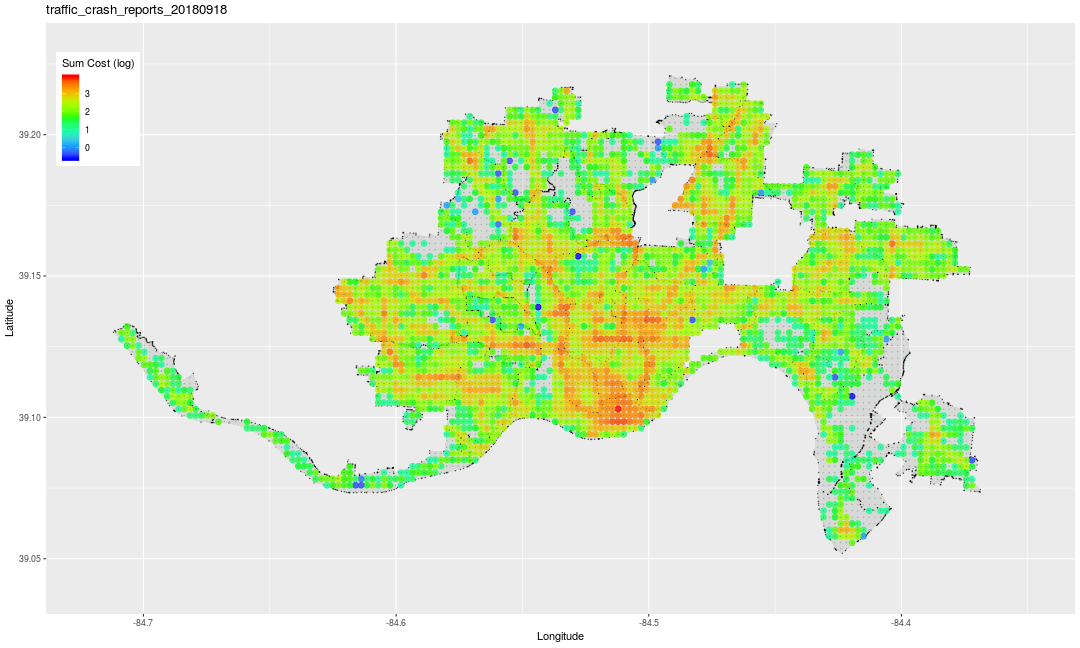
\includegraphics[width=\textwidth, height=\textheight, keepaspectratio]{trafficcrashreports20180918nonpedestriansumcostmapped2grid.png}
 	\caption{Sum cost of traffic crashes reported from 2012 to October 2018 involving pedestrians by grid cells.}
	\label{figure:SumCrashPlot}

\end{figure}
\FloatBarrier

\subsection{Random Forest - Binary Model}

\subsection{Multi-Variate Linear Regression - Cost Model}
In order to create a linear cost model to predict the cost of a PVI, the data must lend itself to the assumptions of a parametric model. These assumptions include normality, linearity, constant variance, and independence. The response variable within the data has a very abnormal distribution, with nearly 80\% of the grid-cells containing no incidents of PVI and having 0 cost associated with them. This positively skewed data does not meet the assumption of normality even after multiple types of transformations, notably including the logarithmic transformation. In order to meet the assumption of normally distributed data, the data is subset to exclude locations where there is no data, and the few events resulting in extreme damage of \$5 million or more. This data subset dramatically reduces the skewness present in the dataset, and allows for linear regression modelling to proceed.

The reduced scope dataset is first run through the 10-fold cross validated stepwise selection of the caret package in R, in order to determine the best full model, ranging from 10 to 35 predictor variables. The function iterates through each number of predictor variables from 10 to 35, performing stepwise 10-fold cross validation for each number of maximum predictor variables. The 10-fold cross validation is a model validation technique used to reduce overfitting and promote the generalizability of the model. Model overfitting can occur when a model is trained on a particular dataset to the degree that it performs extraordinarily well in predicting on the dataset, but it fails to achieve that same level of prediction capability on other datasets. The parameters in an overly fit model do not generalize to the population at large because they are fine tuned to only reflect the dataset on which they were trained. The 10-fold cross validation splits the data into 10 pieces. In each of the 10 iterations, one is selected to be the testing dataset, and the other 9 are used to train the model. This methodology is repeated so that each of the 10 pieces has a chance to be the testing dataset. The result of these 10 trials are averaged and compared against the cross validation results at each other maximum variable value from 10 to 35. The full model chosen is the model with the lowest average root mean square error value, and in our study, was determined to be the model with 30 variables.

Once the full model is selected, it is then manually pruned based on the variance inflation factor values and significance. Variance inflation factor values larger than 5 signify collinearity between variables, and a violation of one of the parametric assumptions in linear regression. Variable significance is determined by the p-value, and the typical value used is .05. Variables at or below the .05 p-value threshold are determined to be statistically significant to the model, while those above it are not. In spite of this black and white view on p-values, some variables are left in the model which are not significant at the .05 level, but are suggestive of being significant influences to the model, as shown in PLACEHOLDER1. 

With the reduced model, the cost of non-fatality incidents to pedestrians is predicted for each event, and the resulting prediction is compared against the actual cost of incident. The difference between the predicted and actual cost is the residual, and the residuals are then mapped back to the Cincinnati map to visualize areas with potential for safety improvement.



\subsection{Non-Supervised Learning - Neighborhood Characterization}



To develop the models in a way that supports an assessment of the generalizability of the models,  the dataset is shuffle split into 80:20, 20\% holdout for cross-validation, using the 10-fold cross-validation stratified shuffle split function from the scikit-learn library for Python. The 80\% is then split into a further 80:20 for training and testing. Machine learning and deep learning algorithms are used as listed in Table ~\ref{table:algorithmsandmethods}. Models are compared with each other on different performance metrics, such as the area under curve and brier score.
%
\FloatBarrier
\begin{table}
\begin{center}
\caption{Algorithms and evaluation methods}
\label{table:algorithmsandmethods}
\begin{tabular}{p{50mm} p{60mm}}
\hline
\rule{0pt}{12pt}
Algorithm	&	Models	\\[2pt]
\hline
Regression 	&	1.        Multiple Regression	
				2.        Support Vector Machine	\newline
				3.        Decision Tree	\\
Unsupervised Learning	&	1.        Clustering	\newline
				\hspace*{5mm} a.        K-means	\newline
				\hspace*{5mm} b.        Hierarchical 	\newline
				2.        Gaussian Mixture Models	\newline
				3.        Neural Networks	\newline
				\hspace*{5mm} a.        Self Organizing Maps	\\
Additional 	&	1.        T-Distributed Stochastic Neighbor Embedding	\newline
				2.        Principal Component Analysis	\newline
				3.        Linear Discriminate Analysis	\newline
				4.        Natural Language Processing	\\[2pt]
\hline
\end{tabular}
\end{center}
\end{table}
\FloatBarrier
%
\section{Results}
%
\subsection{Data aggregation and grid cell assignment}

The results of several of the data sets aggregated and assigned to each respective grid cell are shown in following figures. In summary, the following features were mapped into the grid cells as candidate features to participate in the modeling :

\FloatBarrier
\begin{table}
\begin{center}
\caption{Feature Definition}
\label{table : featureDefinition}
\begin{tabular}{p{50mm} p{60mm}}
\hline
\rule{0pt}{12pt}
Data category & Specific feature definition	\\[2pt]
\hline
Non-pedestrian accidents 		& Number Events \newline
															Sum cost (NSC) for events \\
Pedestrian survey responses & TBD in next update \\
Reported near misses 				& Number events \newline
                                                            Categorical feature counts \\
Street surface areas 				& Surface total length \newline
                                                            Sum lane counts  \\
Walk Scores 								& Max, Mean, Min  \\
Fire incidents 								& TBD in next update  \\
Non-emergency service requests & Sum number requests \newline
                                                                      Categorical feature counts\\ 
Property values \& uses 			& Median prperty values \newline
                                                            Number of property transfers in 10-year period  \\
Public transportation accessibility & Distance to nearest bus stop \\[2pt]
\hline
\end{tabular}
\end{center}
\end{table}
\FloatBarrier
%


Figure ~\ref{figure : maxWalkScores}. \newline
\FloatBarrier
\begin{figure}
 	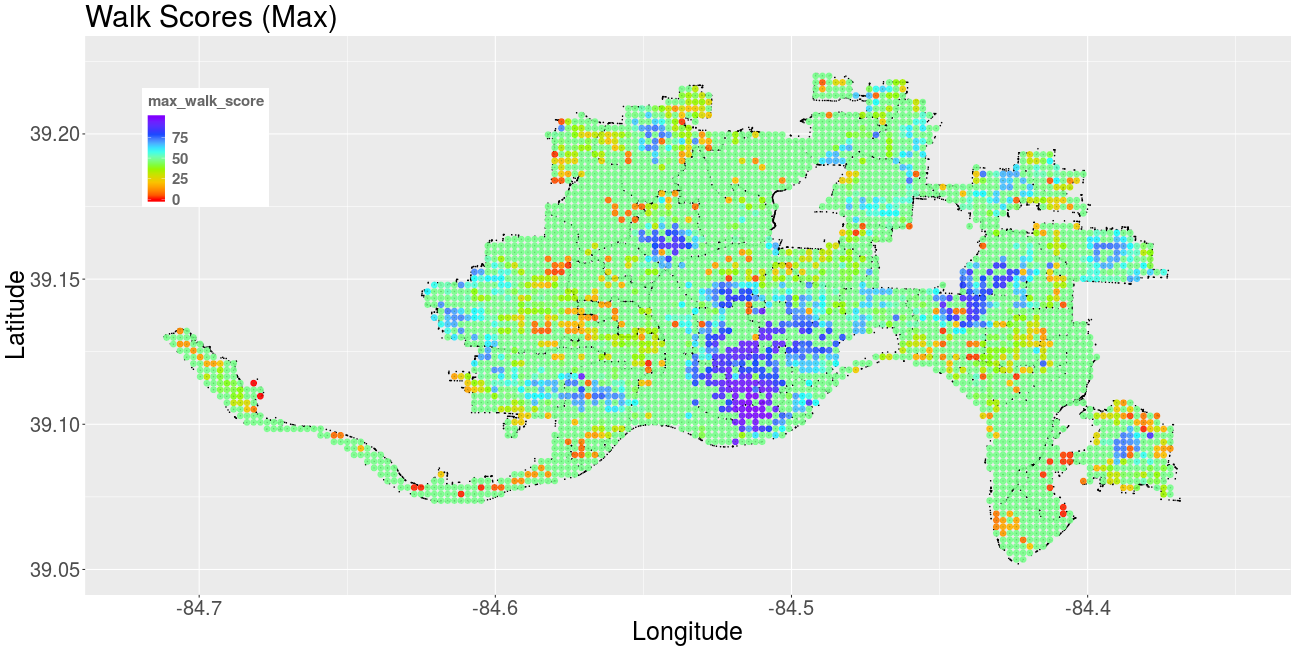
\includegraphics[width=\textwidth, height=\textheight, keepaspectratio]{maxWalkScores.png}
 	\caption{Walk Score - Max values}
	\label{figure : maxWalkScores}
\end{figure}
\FloatBarrier


Figure ~\ref{figure : busStopDistance}. \newline
\FloatBarrier
\begin{figure}
 	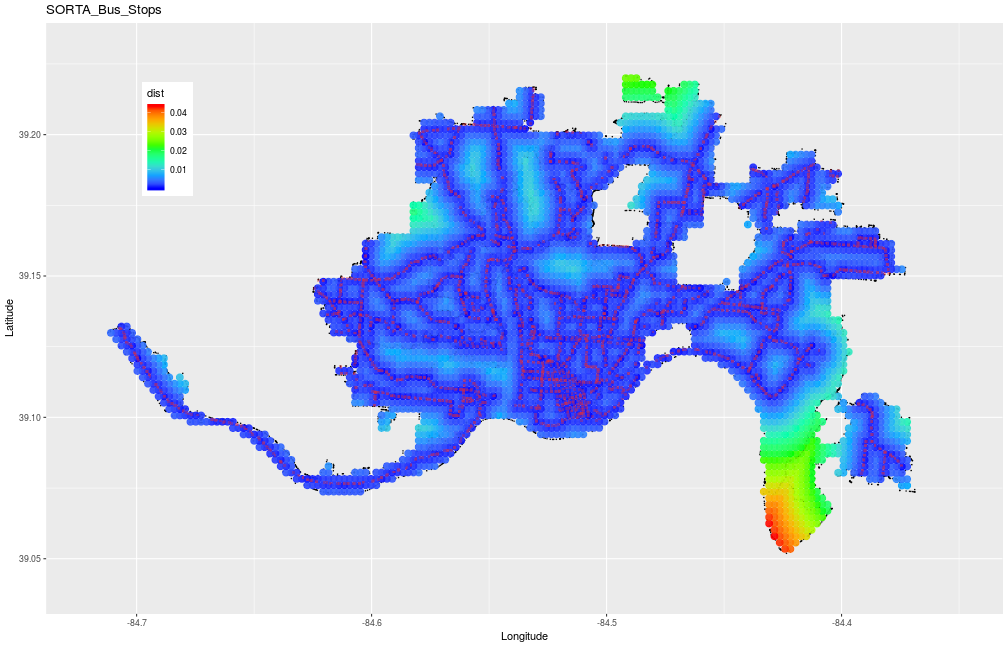
\includegraphics[width=\textwidth, height=\textheight, keepaspectratio]{busStopDistance.png}
 	\caption{Public Transportaton accessibility}
	\label{figure : busStopDistance}
\end{figure}
\FloatBarrier

Figure ~\ref{figure : trafficAccidents}. \newline
\FloatBarrier
\begin{figure}
 	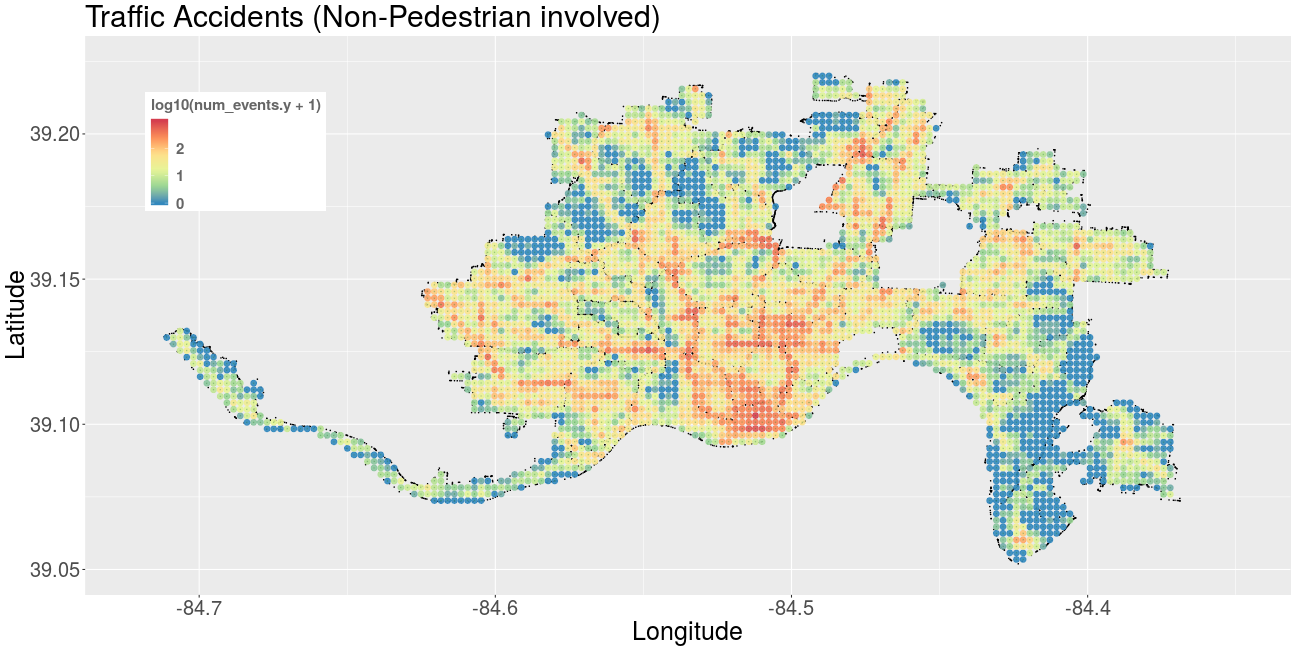
\includegraphics[width=\textwidth, height=\textheight, keepaspectratio]{trafficAccidents.png}
 	\caption{Number of Traffic Accidents (Non-pedestrian involved)}
	\label{figure : busStopDistance}
\end{figure}
\FloatBarrier

\subsection{Random Forest - Binary Model}

The random forest model which we deployed to estimate occurrence of pedestrian related events produces the result of 75\% true positive, 20\% false positive with a detection threshold set at 0.20. This result provides a balanced compromise between true positive and false positive, as depicted in the following Figure ~\ref{figure : rfroccurve}. \newline
\FloatBarrier
\begin{figure}
 	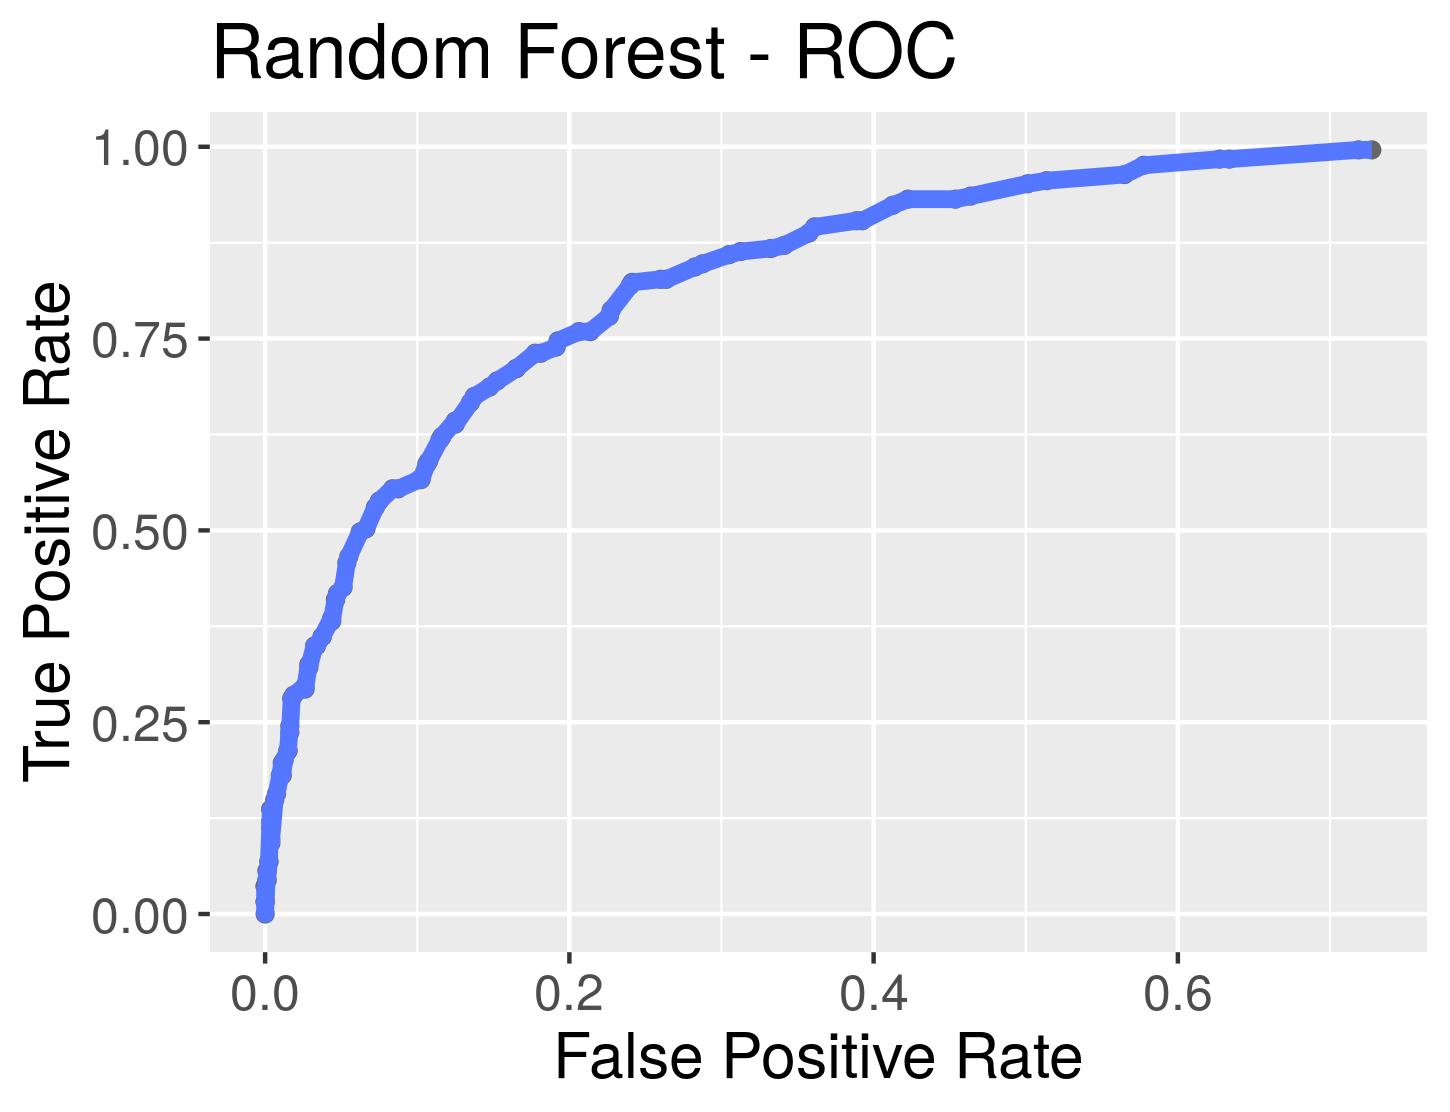
\includegraphics[width=\textwidth, height=\textheight, keepaspectratio]{RFROC.png}
 	\caption{Random forest - binary model - ROC curve}
	\label{figure : rfroccurve}
\end{figure}
\FloatBarrier

As visualized on the map of the city, Figure ~\ref{figure : rfbinarymap}, we observe that (a) the regions of true positve (green) and true negative (light grey) comprise the large majority of the surface area, generally represented by contiguous areas, and confirm the high overall accuracy of the model, (b) that the false positive (darker grey) and false negative (red dots) are consistently along the border regions between otherwise true positive or true negative regions, and (c)  the false negative regions are distinct non-connected grid cells at somewhat widely distributed locations around the city.
\newline

\FloatBarrier
\begin{figure}
 	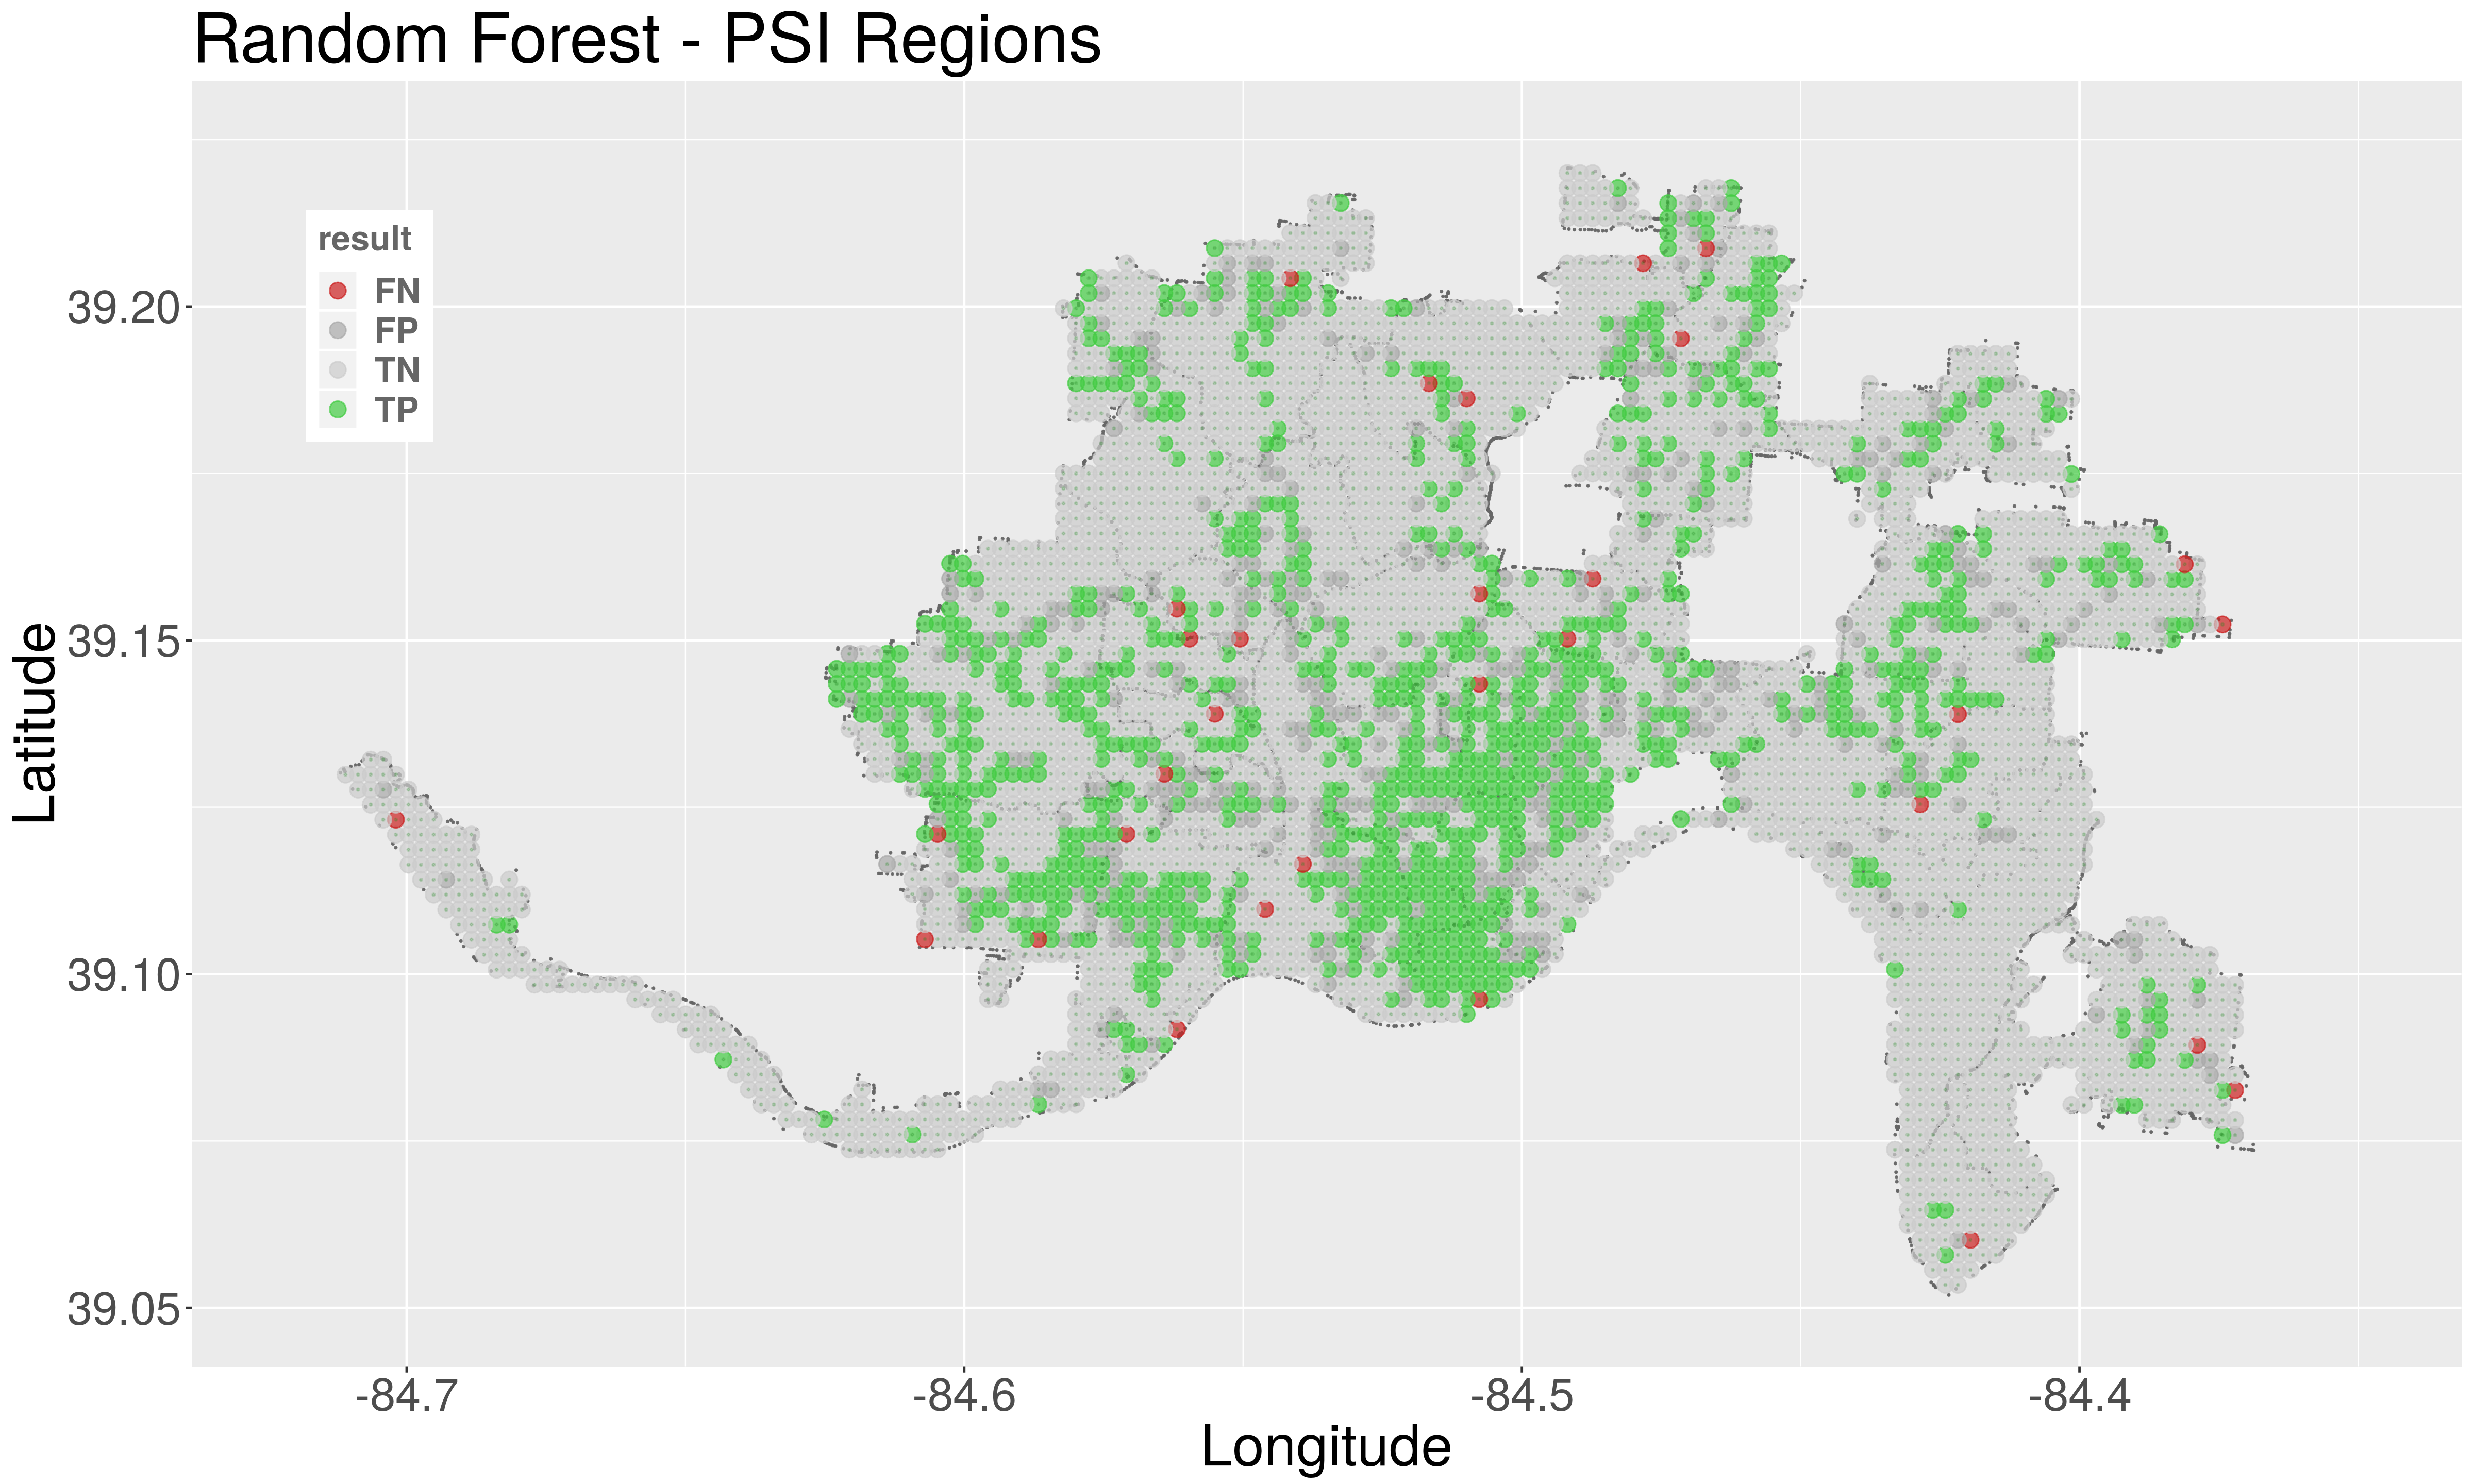
\includegraphics[width=\textwidth, height=\textheight, keepaspectratio]{RFBinaryResultsMap.png}
 	\caption{Distribution of random forest model results visualized on city map}
	\label{figure : rfbinarymap}
\end{figure}
\FloatBarrier

\subsection{Multi-variate linear regression - Cost Model}

\subsection{Non-supervised learning - Neighborhood characterization}

Initial results from part 1 of our methodology have produced graphs as shown in Figure ~\ref{figure:SumCrashPlot}. \newline
\FloatBarrier
\begin{figure}
 	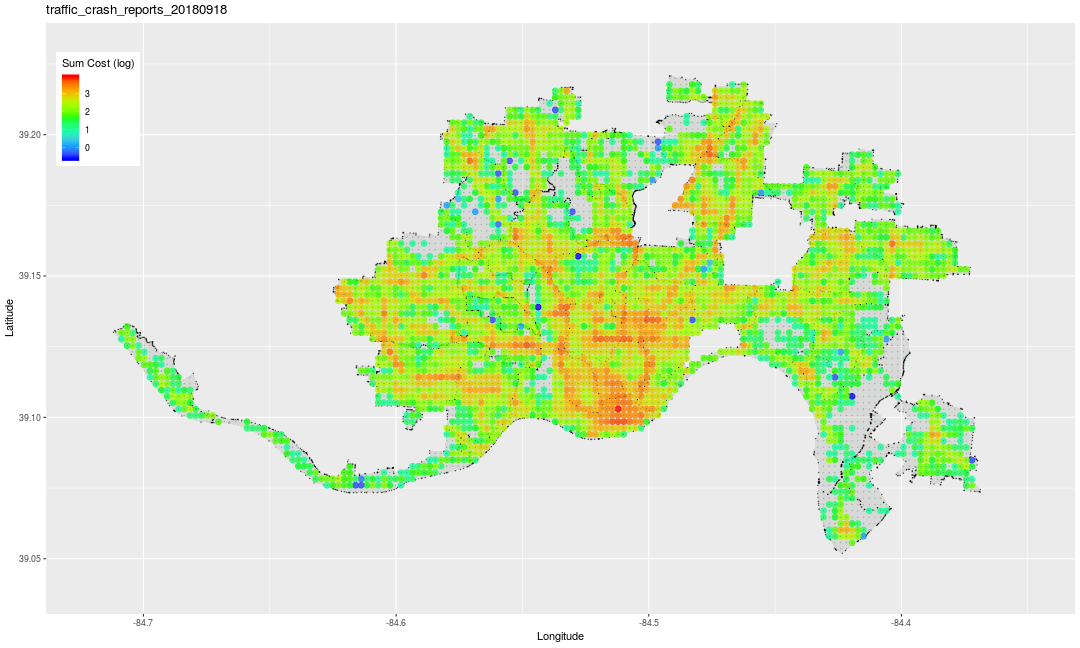
\includegraphics[width=\textwidth, height=\textheight, keepaspectratio]{TrafficCrashReports20180918SumCostMapped2Grid.png}
 	\caption{Sum cost of traffic crashes reported from 2012 to October 2018 involving pedestrians by grid cells.}
	\label{figure:SumCrashPlot}
\end{figure}
\FloatBarrier
%
\section{Analysis}
%
\subsection{Random Forest - Binary Model}

The focus of this effort is to identify locations within the city that indicate highest potential for safety improvement. Consistent with the concept as defined and implemented in other works, the model incidents for which the observed experience exceeds the expected (model output) response are the regions with potential for safety improvement. In the context of a binary model, as was completed here with the random forest model, the regions of PSI are the false negative points on the grid map, as presented in Figure ~\ref{figure : rfbinarymap}. For these grid cells, the model result was no expected pedestrian events, yet the observed experience exceeded this expected response. In this case, there are 31 grid cells identified with potential for safety improvement. In the next update to this draft, we will present what are the unique characteristics of these grid cells, where they are located geographically within the city (street and intersection identification) and what was the ac
%
\section{Results}
%

\subsection{Random Forest - Binary Model}

\subsection{Multi-Variate Linear Regression - Cost Model}

\subsection{Non-Supervised Learning - Neighborhood Characterization}

%
\section{Analysis}
%

\subsection{Random Forest - Binary Model}

\subsection{Multi-Variate Linear Regression - Cost Model}
The results from the prior section provide a numerical and visual way to interpret the model. Because the regression model was subset based on the total cost of damage to the pedestrian excluding events resulting in \$5 million or more in damages, this results in the scope of the model being limited to non-fatality incidents. The regression model is able to explain 20\% of the variance in the cost of a non-fatality incident. This model consists of many significant variables, such as reports of crosswalks needed and reports of vehicles not obeying traffic signs, and some suggestively significant variables which make sense practically, but do not meet the p-value threshold of .05 such as speeding (p-value = .066), parking close to an intersection (p-value = .077), and parking on the sidewalk (p-value = .081). Most variables present within the model are reports to the non-emergency police telephone number, or the city’s online safety survey. For each incident of report within the grid-cell, the predicted total cost of non-fatality incident changes by the estimated amount. Other non-report variables include the number of police properties present within the grid-cell, the maximum Walk Score value of properties within the grid-cell, and the total cost of damage to people involved in non-pedestrian related (motor vehicle) accidents. 

Figure PLACEHOLDER2 illustrates the model’s predictive capability as compared to the cost of incident in reality. Points which are colored in red have positive residuals, meaning the model has underestimated the cost. Green points have negative residuals, which mean the model has overestimated the cost. The further away a point is, the larger its absolute residual value is. These distances are displayed on Fig PLACEHOLDER3, where the red colored areas correspond to the distant red points. These areas within the city in which the model has underestimated the cost the most have the most potential for safety improvement, because all other factors being equal, there is something about that area which is causing a higher amount of damage to pedestrians.

\subsection{Non-Supervised Learning - Neighborhood Characterization}

%
\section{Ethics}
%
As a means to evaluate compliance with ethical considerations, we use the model of the ACM Code of Ethics  (the Code). Within the Code, there are four primary sections, e.g., General Ethical Principles, Professional Leadership Principles, etc., with each primary section providing additional subsections for self-assessment compliance to the Code. For each sub-section, we self-scored categorically as either Y, n/a, or D, where Y indicates that the work completed for this project rather obviously complies with the Code, n/a indicates that that section of the Code is less obviously significant for this project, and D indicates that that section of the Code identifies a potential ethical dilemma that is worthy of additional discussion to demonstrate compliance or at least point out the potential ethical challenge identified from this self-assessment.
The most significant elements that we self-assess as D are : \S 1.2 - Avoid harm; \S 1.4 - Be fair and take action not to discriminate; and \S 3.7 - Recognize and take special care of systems that become integrated into the infrastructure of society.

From these three elements, we consider that the significant question to evaluate is: how may these research findings be interpreted and used ?

The result of this project provides a recommended prioritization for the allocation of municipal resources for the purpose of improving a pedestrian safety problem. Allocation of  public resources is often as much a political challenge as it is a scientific challenge. There is no global objective function that assigns absolute social value to any decision of resource allocation. That is, in fact, the work and challenge of public officials. Within the general framework of public decision making it is recognized that facts, reports, and recommendations which are or were essentially the result of objective research are frequently interpreted in a way that suits the interpreter for their own agenda – in some cases for personal gain – financially or politically. We have to admit for this case, then, that this evaluation is potentially subject to a personally motivated interpretation. The debate about using scientific research to guide public policy is long and continuing. With that recognition, the task falls to us to identify what steps are taken to reduce the risk of unintended uses of this report.

First, the report as written has limited scope for direct application to policy. The recommendations included are applicable to the specific time period and data evaluation associated to the City of Cincinnati. The methods presented here can be widely applied (and in fact, that is the goal of this research), but in current form it would be difficult to justify using these results for direct resource allocation in any other municipality. The model developed here used very specific local experiences – accidents, reported near accidents, local conditions survey, property valuations, social media, and all other elements that contributed to this model are local and specific to the City of Cincinnati and to the current time period. As such, the specific recommendations are not generalizable. The method is generalizable; the specific results may provide indications of what local elements in other municipalities may prove indicative or at least useful for a similar exercise, but in any rational discourse, it would be difficult to extend the specific recommendations from this study to municipalities beyond the extent of this study.

Secondly, this report is submitted to representatives of the Cincinnati City Council and the Department of Safety . By distributing the results to more than one department and to a reasonably broad audience reduces risk of information being used for narrowly scoped  or interests which are not generally aligned with good public discussion, debate, and utilization. Further, the data and methods deployed here were developed based on early and continuing input from representatives of these multiple departments within the City. Thus, early and often participation of multiple stakeholders provided the opportunity to have balanced input to the research, thus improving likelihood of balanced output and utilization. And, by respecting and incorporating the input from multiple perspectives from within the City provides higher likelihood of acceptance (and perhaps adoption) of the resulting recommendations.

Thirdly, within the City of Cincinnati, there are currently several on-going initiatives dedicated to improving pedestrian safety. The other initiatives are, in some cases, significantly funded, and are the work product of several departments within the City, predominantly the Department of Safety, that are the prime stakeholders in promoting public safety in the City. These other initiatives are an order of magnitude more significant, both from resource commitment, and for intended impact, than is this study. It is not our aim to minimize the potential impact of the recommendations from this study, but we are cognizant of the relative significance of this study within the larger context of the on-going programs within the City. In any decision making forum for the City, we consider the likelihood of these results having the capability to be used for unintended or inappropriate outcomes to be sufficiently unlikely.

The ethical considerations associated to this project are adequately assessed in the spirit of the ACM Code. The identified risks are appropriately mitigated.
%
\section{Conclusions (and Future Work)}
%

This study demonstrates a methodology to identify areas within the city of Cincinnati, Ohio with the largest potential for safety improvement, based on many open-source datasets made public by the city. Over twenty 250 meter by 250 meter plots of land within the city have been identified for further investigation to determine why the cost of incident within that area are abnormally high as compared to our models. These locations include several areas in the Westwood neighborhood, Clifton, Avondale, Walnut Hills, Bond Hill, and more. Our unsupervised learning techniques…PLACEHOLDER SENTENCES ABOUT HOW OUR UNSUPERVISED LEARNING TECHNIQUES HAVE OUTLINED AREAS WHICH HAVE POTENTIAL FOR SAFETY IMPROVEMENT. THESE AREAS DEMONSTRATE THESE QUALITIES WHICH ARE RELATED TO PEDESTRIAN SAFETY IN THE CITY OF CINCINNATI OHIO.

Future work to further this project could involve the use of other regression modelling techniques to improve accuracy, such as tobit models. Other improvements which could be made include STUFF GOES HERE FROM PATRICK AND PREETI ABOUT WAYS TO IMPROVE YOUR TECHNIQUES AND MODELS.

Aside from improving the models through the use of different techniques, the study itself can be improved by ingesting more data. This study is carried out using publicly available data, if private data exists which can improve the study, it can easily be adapted for use due to only requiring a street address or latitude longitude coordinates which would allow the data to be integrated into the grid-cell aggregation function. Examples of data which may be useful but are not publicly available would be the race, gender and age of the perpetrator and pedestrian victim, data which the city of Cincinnati may have, though the ethical implications of using this data must be weighed. 

% ---- Bibliography ----
%
\bibliographystyle{splncs}
\bibliography{pedestrianreferences}

\end{document}